In this section we review the flight mechanic principles necessary for understanding our work. We show derivations for calculating the following: \begin{enumerate}
    \item $P_{req}$ - the power required to maintain level flight 
    \item $V_{mp}$ - the linear velocity where $P_{req}$ is minimized.
    \item $P_{req_{turn}}$ - the power required to maintain a level turn
\end{enumerate} Additionally, we show that for level flight $V_{mp}$ is equivalent to the velocity that maximizes endurance.

\subsection{Power Required $P_{req}$}
Using the standard quadrotor model given in \cite{hoffmann2004stanford} and \cite{pounds2002design} with the coordinate frames illustrated in \ref{QuadDiagram} a simple force balance shows that the pitch angle, $\theta$, can be written as a function of $V$. Assuming a windless environment we can say $V = V_\infty$, the relative velocity of the flow, and write \eqref{ThetaOfV}.

\begin{equation}
    \label{ThetaOfV}
    \theta(V_\infty) = \frac{\rho v_\infty^2 f}{2mg}
\end{equation}

\subsection{Equations Likely Needed}

\begin{equation}
    \label{LevelFlightEqn}
    P_{req} = \frac{k T^2}{2\rho A V_\infty}+(\frac{1}{2}\rho V_\infty^2 S_{ref} C_{D_f})V_\infty
\end{equation}

% \begin{figure}[ht]
% 	\centering
% 	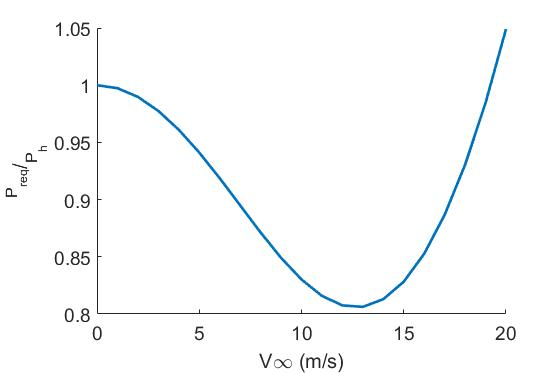
\includegraphics[width=8cm]{constant-config-ratio.jpg}
% 	\caption{The ratio of power required in forward, level flight at a given velocity to power required at hover. Maximum endurance is achieved at the minimum of this curve. For the given configuration we see that flying at $V_{me}$ reduces the power required by 19 percent.}
% \end{figure}

\begin{figure}
    \centering
    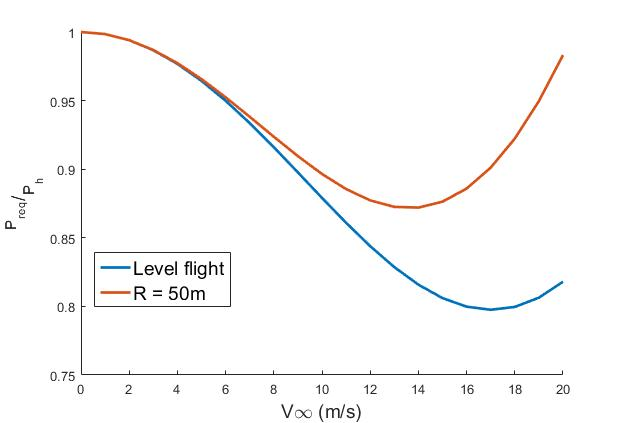
\includegraphics[width=8cm]{images/m100-turn-vs-level.jpg}
    \caption{We compare the theoretical power ratio for our vehicle configuration using momentum theory analysis. If our vehicle was flown straight and level at 17m/s we could expect to fly approximately 21\% longer. Even with losses associated with overcoming centripetal acceleration we can expect to fly 13\% longer by flying at 13m/s while turning with a radius of 50m.}
    \label{m100levelturn}
\end{figure}